% fig-i-1.tex — I.1: equilateral triangle on a given segment.
\begin{figure}[H]
\centering
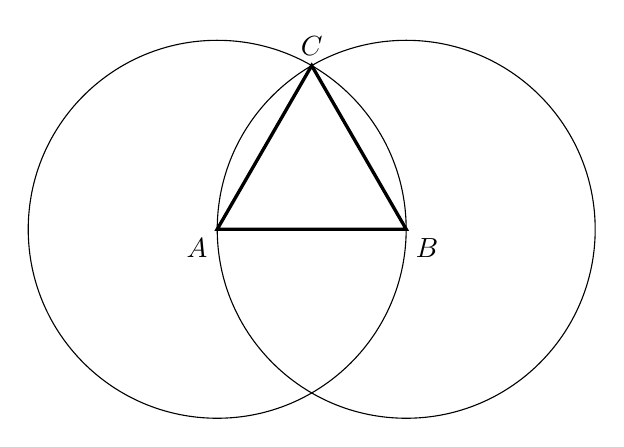
\begin{tikzpicture}[scale=1.2, line cap=round]
  \coordinate (A) at (0,0);
  \coordinate (B) at (2,0);
  \coordinate (C) at (1,{sqrt(3)});
  % Two circles, centres A and B, radius AB.
  \draw[thin] (A) circle (2);
  \draw[thin] (B) circle (2);
  % Triangle.
  \draw[very thick] (A) -- (B) -- (C) -- cycle;
  % Labels.
  \node[below left]  at (A) {$A$};
  \node[below right] at (B) {$B$};
  \node[above]       at (C) {$C$};
\end{tikzpicture}
\caption{Proposition I.1. The two circles with centres $A$ and $B$ and
common radius $AB$ meet at $C$; the triangle $ABC$ is equilateral.}
\label{fig:I.1}
\end{figure}
